\documentclass{article}\usepackage{graphicx, color}
%% maxwidth is the original width if it is less than linewidth
%% otherwise use linewidth (to make sure the graphics do not exceed the margin)
\makeatletter
\def\maxwidth{ %
  \ifdim\Gin@nat@width>\linewidth
    \linewidth
  \else
    \Gin@nat@width
  \fi
}
\makeatother

\IfFileExists{upquote.sty}{\usepackage{upquote}}{}
\definecolor{fgcolor}{rgb}{0.2, 0.2, 0.2}
\newcommand{\hlnumber}[1]{\textcolor[rgb]{0,0,0}{#1}}%
\newcommand{\hlfunctioncall}[1]{\textcolor[rgb]{0.501960784313725,0,0.329411764705882}{\textbf{#1}}}%
\newcommand{\hlstring}[1]{\textcolor[rgb]{0.6,0.6,1}{#1}}%
\newcommand{\hlkeyword}[1]{\textcolor[rgb]{0,0,0}{\textbf{#1}}}%
\newcommand{\hlargument}[1]{\textcolor[rgb]{0.690196078431373,0.250980392156863,0.0196078431372549}{#1}}%
\newcommand{\hlcomment}[1]{\textcolor[rgb]{0.180392156862745,0.6,0.341176470588235}{#1}}%
\newcommand{\hlroxygencomment}[1]{\textcolor[rgb]{0.43921568627451,0.47843137254902,0.701960784313725}{#1}}%
\newcommand{\hlformalargs}[1]{\textcolor[rgb]{0.690196078431373,0.250980392156863,0.0196078431372549}{#1}}%
\newcommand{\hleqformalargs}[1]{\textcolor[rgb]{0.690196078431373,0.250980392156863,0.0196078431372549}{#1}}%
\newcommand{\hlassignement}[1]{\textcolor[rgb]{0,0,0}{\textbf{#1}}}%
\newcommand{\hlpackage}[1]{\textcolor[rgb]{0.588235294117647,0.709803921568627,0.145098039215686}{#1}}%
\newcommand{\hlslot}[1]{\textit{#1}}%
\newcommand{\hlsymbol}[1]{\textcolor[rgb]{0,0,0}{#1}}%
\newcommand{\hlprompt}[1]{\textcolor[rgb]{0.2,0.2,0.2}{#1}}%

\usepackage{framed}
\makeatletter
\newenvironment{kframe}{%
 \def\at@end@of@kframe{}%
 \ifinner\ifhmode%
  \def\at@end@of@kframe{\end{minipage}}%
  \begin{minipage}{\columnwidth}%
 \fi\fi%
 \def\FrameCommand##1{\hskip\@totalleftmargin \hskip-\fboxsep
 \colorbox{shadecolor}{##1}\hskip-\fboxsep
     % There is no \\@totalrightmargin, so:
     \hskip-\linewidth \hskip-\@totalleftmargin \hskip\columnwidth}%
 \MakeFramed {\advance\hsize-\width
   \@totalleftmargin\z@ \linewidth\hsize
   \@setminipage}}%
 {\par\unskip\endMakeFramed%
 \at@end@of@kframe}
\makeatother

\definecolor{shadecolor}{rgb}{.97, .97, .97}
\definecolor{messagecolor}{rgb}{0, 0, 0}
\definecolor{warningcolor}{rgb}{1, 0, 1}
\definecolor{errorcolor}{rgb}{1, 0, 0}
\newenvironment{knitrout}{}{} % an empty environment to be redefined in TeX

\usepackage{alltt}
\usepackage[margin=1.5in]{geometry}
\usepackage{algorithm}
\usepackage{color}
\usepackage{algpseudocode}
\usepackage{amsmath}
\usepackage{url}


\newcommand{\todo}[1]{
    \addcontentsline{tdo}{todo}{\protect{#1}}
    \textcolor{red}{#1}
}

\begin{document}



\title{Hippocampal segmentation with MAGeT}
\author{Jon Pipitone, }
\maketitle

\section{Introduction}

The hippocampus is of particular interest to many researchers because it is implicated in forms of brain dysfunction such as Alzheimer's disease and schizophrenia, and has functional significance in cognitive processes such as learning and memory.  For many research questions involving neuroimaging data, accurate identification of the hippocampus and its subregions in participant MR images is a necessary first step in order to analyse neuroanatomical differences and changes in  sample populations.  \todo{expand}

Currently, the gold standard for neuroanatomical segmentation is manual labelling by an expert human rater.  This is problematic for several reasons.  Practically, manual segmentation takes a significant investment of time and expertise (Hammers2003) which may not be readily available to researchers or clinicians.  <blah> estimates that expert segmentation can take anywhere between 45 minutes to several days per image depending on the image resolution and protocol.  The amount of data produced in neuroimaging experiments increasingly exceeds the capacity for identification of specific neuroanatomical structures by an expert manual rater.  It may be difficult for laboratories to find or train, someone with the expertise to do such segmentation.  

Compounding this is that the hippocampus is a problematic structure for segmentation. Its very definition is disputed and varies widely in the literature (Geuze2004).  This has led to a variety of competing segmentation protocols in the literature which researchers can adhere to, including necessary ad-hoc modifications to adapt the definition in order to answer a particular research question.  Efforts are underway to create a unified protocol (Jack2011) for volumetry applications. But, even with a unified protocol, in order to investigate certain research questions it may be necessary to select from different hippocampal definitions. For example, (Poppenk2011) found that overall hippocampal volume change did not predict recollection memory performance, but dividing the hippocampus into anterior and posterior regions did. 

\todo{this bit needs to be a little clearer - was it just the division of the HC that led to the improved understanding or was it that spatially localized differences in volumes are a better way to describe the difference).}
  
\todo{- Also, other situations: developmental studies -- need different definitions depending on the age range of subjects
-- additionally, may want to tweak definition to test certain hypotheses (e.g. include subiculum: yes/no, more or less 
 conservative WM/GM boundaries, compare with definitions from a different study,, etc...).}

One can also expect neuroanatomical variability in this structure as it loses volume through aging and in the time course of different diseases.  \todo{This bit isn't really "joined to the previous statement"  may need a little glue here}


Automated segmentation techniques are available and can minimize several of the confounds often observed in studies that involve manual volumetry, such as the time and expertise required for segmentation and intra- and inter-rater reliability.  A class of segmentation approaches, known as atlas-based segmentation (also, template-based segmentation), make use of expertly labeled neuroanatomical atlases. An atlas MR image is warped to fit the subject neuroanatomy using nonlinear registration techniques [4, 11], and then the atlas labels are propagated via the registration transformation from the atlas to match the unique neuroanatomy of a particular subject.  Segmentation accuracy is affected by nonlinear registration and resampling errors, and by the extent to which the atlas neuroanatomy differs from the underlying neuroanatomical variability of the population under study (citation needed).  To address these limitations, several atlases can be used (multi-atlas segmentation). Labels from each atlas are propagated to the subjects, by way of an nonlinear image registration, producing as many labellings for each subject as atlases. A label fusion technique is employed to merge the candidate labellings for a subject into a single segmentation using a decision rule (for instance, voxel-wise voting). Not all of the atlases need be used to segment each subject. Selecting only those atlases that are most similar to the subject image has been shown to significantly improve overall registration and segmentation accuracy (Aljabar 2008, Collins2010, Leung2010, Lotjonen2010). 

\todo{briefly discuss other automated segmentation methods, and justify our focus on atlas-based methods}

In summary, whilst manual segmentation is the gold standard for neuroanatomical segmentation, it is time-consuming and requires an investment in expertise and training, and may be inflexible in the face of differing hippocampal definitions or changes. Atlas-based automated segmentation dramatically reduces the time needed for segmentation, and can be completed without any expert rater as long as an appropriate atlas library is available <be more specific (e.g. shares protocol, demographics, phenotypes of subject population)>.  In the situation where such an atlas library does not exist, then an expert rater is needed. Many automated approaches rely on an atlas library containing between 30 and 80 expertly labeled brains (Heckemann2006, Collins2010) which, even though producing such a library may require less manual work than segmenting the entire set of subjects, it still poses a substantial time commitment.  

In this paper we extend our automated method for subcortical segmentation (striatum, globus pallidus, and thalamus; Chakravarty2012) to hippocampal segmentation. This method, known as MAGeT brain, is suited for situations where manual effort is at a premium, and flexibility is needed in atlas definitions.  Our strategy is to bootstrap the familiar multi-atlas-based segmentation process from only a very small number of atlases.  In our previous work we used only a single atlas, based on serial histological slices, and validated the algorithm on 20 adolescent MR images.  In this work, we extensively investigate MAGeT used with differently sized atlas and template libraries, registration algorithms, label fusion strategies, and hippocampal definitions.  We evaluate our algorithm on a subset of images from the ADNI dataset, and compare our segmentations to the manual segmentations provided by ADNI.  Additionally, we evaluate the segmentations produced with MAGeT using hippocampal definitions from five high-resolution T1 in-vivo atlases (Winterburn2012). <conclude with summary that this is detailed validation the algorithm in order to pick the best operating parameters, whereas our previous work showed the feasibility of the approach> 

The essential insight of MAGeT brain, generating a template library, is not new. Heckemann2006 compared a multi-atlas-based segmentation method to that of generating a template library from a single atlas and found poor performance so did not investigate this approach any further. The LEAP algorithm (Wolz2010) begins with 30 atlases and labels the most similar unlabeled images. The labeled images from this step are included in the atlas set for the following step, and this proceeds until all images have been labeled. <expand; include other multi-atlas methods too? >

In this work we conduct a thorough validation of the MAGeT brain approach. Our aim is not to improve on segmentation accuracy beyond existing methods, but instead to provide a method that trades off manual segmentation expertise for computational processing time whilst providing useful accuracy for the research and clinical setting. <blah blah.. this sucks>

\section{Materials and Methods}
explain two registration methods, definitions, fusion methods. 
compare to each other, and then compare atlas-based, true multi-atlas, naive methods.
trying to make choices as to the best reg/fusion/

evaluations
described previously in Chakravarty2012. 

\subsection{Segmentation Algorithm}
The segmentation approach we follow is an extension of traditional multi-atlas segmentation. In multi-atlas segmentation, the inputs are a template library consisting of a set of manually labelled MR images (atlases), and a set of unlabelled MR images to be labelled.  Each unlabelled MR image is segmented by first propagating to it the labels from the template library images via image registration, and then these candidate labels are combined by a label fusion method (e.g. voxel-wise majority voting). The label fusion method used may determine which templates are used to segment a particular subject (for instance, voxel-wise majority vote takes labels from all templates, whereas a weighted majority vote selects only those templates most similar to the subject). 

Our extension to this approach is to add a preliminary stage in which we construct the template library using a much smaller set of atlases and a subset of the given unlabelled images.  To begin, we (possibly arbitrarily) select from the unlabelled images to form the template library.  Multiple labellings are given to each image in the template library via label propagation from each of the atlases (label fusion is not conducted).  Traditional multi-atlas segmentation is then used to produce segmentations for the entire set of unlabelled images (including those used in the template library).  Our algorithm is illustrated in pseudocode in Algorithm 1, and diagrammatically in Figure 1. 

- Essentially, we add an extra layer of label propagation between the set of atlases 
- This allows the template library to better reflect the constitution of the images to be labelled.

Source code can be found at \url{http://github.com/pipitone/MAGeTbrain}.

\begin{algorithm}
\caption{Pseudocode for the MAGeT Brain algorithm}
\label{pseudocodesdf}
\begin{algorithmic}
\Function{MultiAtlas}{Templates, Subjects}
  \ForAll{$subject$}
    \ForAll{$template$}
      \State propagate all labels for template to subject space
      \State store subject labels
    \EndFor
    \State fuse subject labels
  \EndFor
\EndFunction
\\
\Function {MAGeTBrain}{Subjects, Atlases, n}
  \For{$i = 1 \to n$}
    \State choose a subject to be used as a template
    \State propagate labels from each atlas to template space
    \State store the template with all of its labels
  \EndFor
  \State MultiAtlas(Templates, Subjects)
\EndFunction
\end{algorithmic}
\end{algorithm}

\begin{figure}[h]
  \centering
    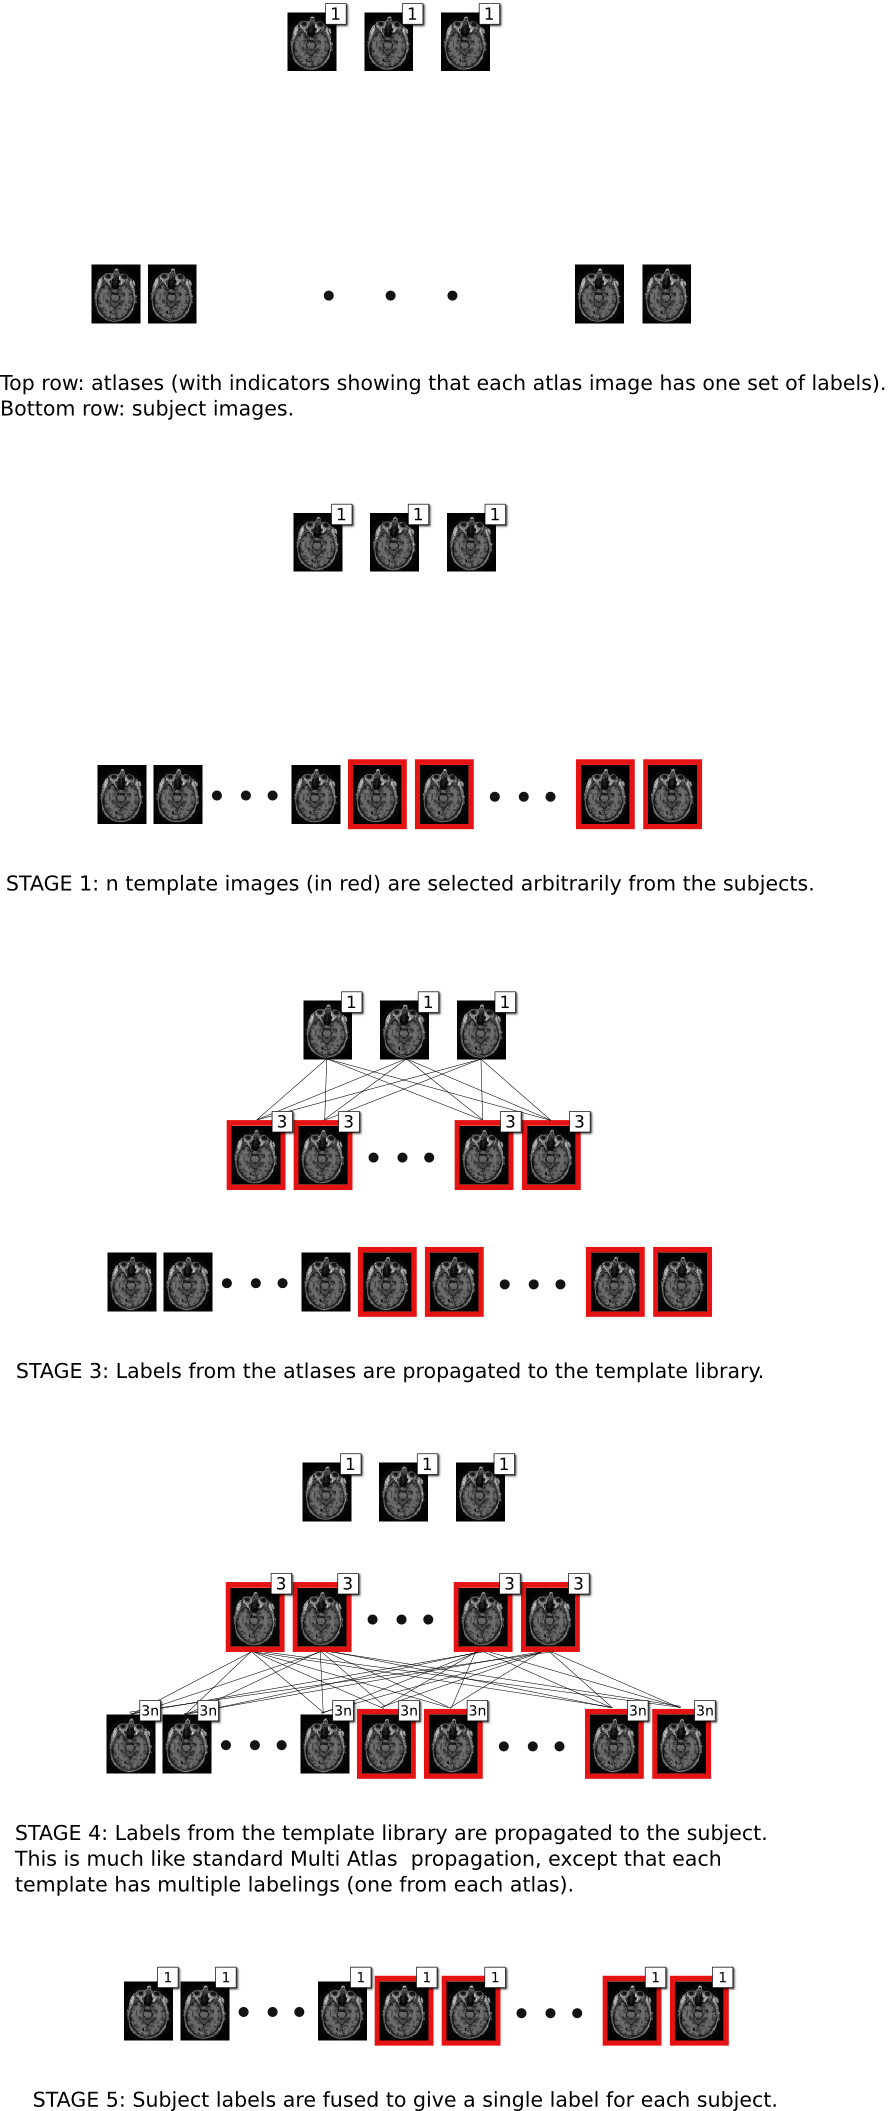
\includegraphics[width=0.5\textwidth]{MAGeT-figure.png}
  \caption{Diagram of the MAGeT Brain algorithm}
\end{figure}

\subsection{Image Processing and Registration Methods}

Before images were registered, the N3 algorithm [16] is first used to minimize the intensity nonuniformity in each of the atlases and unlabeled subject images. In this work we investigated the performance of two registration methods.  

\subsubsection{Automatic Normalization and Image Matching and Anatomical Labeling (ANIMAL)}

The ANIMAL algorithm carries out Image registration is in two phases. In the first, a 12-parameter linear transformation (3 translations, rotations, scales, shears) is estimated between images using an algorithm that maximizes the correlation between blurred MR intensities and gradient magnitude over the whole brain [3]. In the second phase, nonlinear registration is completed using the ANIMAL algorithm [4]: an iterative procedure that estimates a 3D deformation field between two MR images. At first, large deformations are estimated using blurred version of the input data. These larger deformations are then input to subsequent steps where the fit is refined by estimating smaller deformations on data blurred with a Gaussian kernel with a smaller FWHM. The final transformation is a set of local translations defined on a bed of equally spaced nodes that were estimated through the optimization of the correlation coefficient. 
\todo{should add the MNI website here; also we should add the parameters we used somewhere}

\subsubsection{Automatic Normalization Tools (ANTS)}

ANTs is a diffeomorphic registration algorithm which provides great flexibility over the choice of transformation model, objective function, and the consistency of the final transformation. The transformation is estimated in a hierarchical fashion where the MRI data is subsampled, allowing large deformations to be estimated and successively refined at later hierarchical stages (where the data is subsampled to a finer grid). The deformation field and the objective function are regularized with a Gaussian kernel at each level of the hierarchy. The ANTs algorithm is freely available \url{http://www.picsl.upenn.edu/ANTS/}. We used an implementation of the ANTS algorithm compatible with the MINC data format, mincANTS \url{https://github.com/vfonov/mincANTS} \todo{(same here we should add the parameters we used).}

\subsection{Label Fusion Methods}

Label fusion is term given to the process of combining the information from several candidate labellings for an MR image into a single labelling.  In this paper we explore the benefits of three different fusion methods. 

\subsubsection{Voxel-wise Majority Vote}

Labels are propagated from all template library images to a subject.  Each output voxel is given the most frequent label at that voxel location amongst all candidate labellings.  Ties are broken arbitrarily.

\subsubsection{Cross-correlation Weighted Majority Vote}

Labels are propagated from only those template library images which most similar to the subject.  
A voxel-wise majority vote is carried out from the labels from the top n ranked template library 
images, where n is parameter set by the user. 

Similarity between a subject and a template image is measured using normalized cross-correlation of intensity values, over a region of interest defined on each template, after the subject has been linearly registered to the template. The heuristic used for defining a meaningful region of interest for each template is to use the extent of all the propagated labellings from each atlas (after linear registration only) and then dilating this region by three voxels.
 
The utility to calculate the cross-correlation similarity measure is implemented as part of the ANIMAL toolkit. \todo{(ANIMAL or MINC)}

\subsubsection{Normalised Mutual Information Weighted Majority Vote}

This label fusion method is identical to the above process except a normalised mutual information score is used over the region of interest between a template and subject instead of cross-correlation.  

The utility to calculate the normalised mutual information measure is implemented as part of the EZMinc package (based on ITK NMI routine).

\subsection{Goodness-of-fit}

Each segmentation was evaluated against the 'gold-standard' manual segmentation from the dataset using the Dice Kappa ($\kappa$) overlap metric:

\begin{equation*} 
\kappa=\frac{2a}{2a+b+c}
\end{equation*}

where $a$ is the number of voxels common to the candidate segmentation and the gold standard and $b+c$ is the sum of the voxels uniquely identified by either the automatically generated candidate segmentation or the gold-standard. \todo{I would do this after you define the experiments}

\subsection{Data and Experiments}

Three different experiments were conducted to evaluate the influence of registration method, atlas set size and resolution, template set size, and label fusion method and parameters.

\subsubsection{ADNI Validation Experiment}

In this experiment we performed repeated random sub-sampling cross-validation of the MAGeT algorithm with a pool of 69 images and labels from the ADNI dataset.  The images are T1-weighted \todo{<insert description of scan/machine types>}.  The hippocampal labels are provided as part of the ADNI dataset, and are produced \todo{<insert description of SNT labellings>}.  The parameters we varied, and the ranges over which we varied are listed in \todo{table}.  We performed 10 validations per parameter combination.  In each validation trial, a random sample of subjects were chosen from the pool without replacement as the atlas set, whereas the template set was chosen randomly with replacement.   

\begin{table}
    \begin{tabular}{l|l}
        Parameter           & Values tested                                                      \\ \hline
        Number of Templates & 3 to 20                                                            \\ 
        Number of Atlases   & 3 to 9                                                             \\ 
        Registration Method & ANTS or ANIMAL                                                     \\ 
        Label Fusion Method & majority vote, cross-correlation weighted vote, NMI weighted vote. 
    \end{tabular}
\end{table}

We used the following parameters for ANTS, during registration: 
\begin{verbatim}
  mincANTS 3 -m PR[target_file.mnc,source_file.mnc,1,4] 
   --number-of-affine-iterations 10000x10000x10000x10000x10000 
   --affine-gradient-descent-option 0.5x0.95x1.e-4x1.e-4
   --use-Histogram-Matching --MI-option 32x16000
   -r Gauss[3,0] -t SyN[0.5] -i 100x100x100x20
   -o transformation.xfm
 \end{verbatim}
These settings were adapted from the "reasonable starting point" given in the ANTS manual. \todo{<rationale?>}

For the purposes of this work we used the regularization parameters optimized in Robbins et al.[15]. \todo{right? (but added a second layer).}

\todo{multi-atlas comparison, "naive" comparison}

\subsubsection{Winterburn High-resolution Hippocampal Atlas - ADNI Validation}

In this experiment we explored using the MAGeT brain algorithm with the Winterburn high-resolution atlases to segment 21 randomly chosen MR images from the ADNI dataset (seven each of healthy, MCI and AD subjects).  The Winterburn atlases are digital segmentations of the hippocampus in five  in-vivo 300u isotropic T1-weighted MR scans, and include subfield segmentations for the cornus ammonis (CA) 1, CA4, dentate gyrus, subiculum, and CA 2 and 3 combined.  Subjects in the Winterburn atlases range in age from 29-57 years (mean age of 37), and include two males and three females.  

Since hippocampal segmentation protocols differ between the ADNI labels and Winterburn atlases, this poses a problem for direct similarity comparisons between labels produced by MAGeT brain and the ADNI labels.  \todo{explain why we did(n't) resegment the ADNI images with a the low-res protocol.} To evaluate the performance of MAGeT brain, we compared classification accuracy of subjects by diagnosis based on hippocampal volume using both the SMT labels and our produced labels.  \todo{description of validation -- rms {\tt validate} or t-test: contrast with QDA or LDA (Coupe 2011) used in LOOCV}

\todo{For minctracc -- we registered to TAL}

\subsection{Results}
\subsubsection{A2A}

Kappa vs. Number of templates: 
Smoothing line fitted using GAM (generalised additive model) from R with defaults from ggplot2 (formula: y ~ s(x, bs = "cs"))

\begin{knitrout}
\definecolor{shadecolor}{rgb}{0.969, 0.969, 0.969}\color{fgcolor}\begin{kframe}


{\ttfamily\noindent\itshape\textcolor{messagecolor}{\#\# geom\_smooth: method="auto" and size of largest group is >=1000, so using gam with formula: y \textasciitilde{} s(x, bs = "cs"). Use 'method = x' to change the smoothing method.}}

{\ttfamily\noindent\itshape\textcolor{messagecolor}{\#\# geom\_smooth: method="auto" and size of largest group is >=1000, so using gam with formula: y \textasciitilde{} s(x, bs = "cs"). Use 'method = x' to change the smoothing method.}}

{\ttfamily\noindent\itshape\textcolor{messagecolor}{\#\# geom\_smooth: method="auto" and size of largest group is >=1000, so using gam with formula: y \textasciitilde{} s(x, bs = "cs"). Use 'method = x' to change the smoothing method.}}

{\ttfamily\noindent\itshape\textcolor{messagecolor}{\#\# geom\_smooth: method="auto" and size of largest group is >=1000, so using gam with formula: y \textasciitilde{} s(x, bs = "cs"). Use 'method = x' to change the smoothing method.}}

{\ttfamily\noindent\itshape\textcolor{messagecolor}{\#\# geom\_smooth: method="auto" and size of largest group is >=1000, so using gam with formula: y \textasciitilde{} s(x, bs = "cs"). Use 'method = x' to change the smoothing method.}}

{\ttfamily\noindent\itshape\textcolor{messagecolor}{\#\# geom\_smooth: method="auto" and size of largest group is >=1000, so using gam with formula: y \textasciitilde{} s(x, bs = "cs"). Use 'method = x' to change the smoothing method.}}\begin{verbatim}
## pdf 
##   2
\end{verbatim}


{\ttfamily\noindent\itshape\textcolor{messagecolor}{\#\# geom\_smooth: method="auto" and size of largest group is >=1000, so using gam with formula: y \textasciitilde{} s(x, bs = "cs"). Use 'method = x' to change the smoothing method.}}

{\ttfamily\noindent\itshape\textcolor{messagecolor}{\#\# geom\_smooth: method="auto" and size of largest group is >=1000, so using gam with formula: y \textasciitilde{} s(x, bs = "cs"). Use 'method = x' to change the smoothing method.}}

{\ttfamily\noindent\itshape\textcolor{messagecolor}{\#\# geom\_smooth: method="auto" and size of largest group is >=1000, so using gam with formula: y \textasciitilde{} s(x, bs = "cs"). Use 'method = x' to change the smoothing method.}}

{\ttfamily\noindent\itshape\textcolor{messagecolor}{\#\# geom\_smooth: method="auto" and size of largest group is >=1000, so using gam with formula: y \textasciitilde{} s(x, bs = "cs"). Use 'method = x' to change the smoothing method.}}

{\ttfamily\noindent\itshape\textcolor{messagecolor}{\#\# geom\_smooth: method="auto" and size of largest group is >=1000, so using gam with formula: y \textasciitilde{} s(x, bs = "cs"). Use 'method = x' to change the smoothing method.}}

{\ttfamily\noindent\itshape\textcolor{messagecolor}{\#\# geom\_smooth: method="auto" and size of largest group is >=1000, so using gam with formula: y \textasciitilde{} s(x, bs = "cs"). Use 'method = x' to change the smoothing method.}}\end{kframe}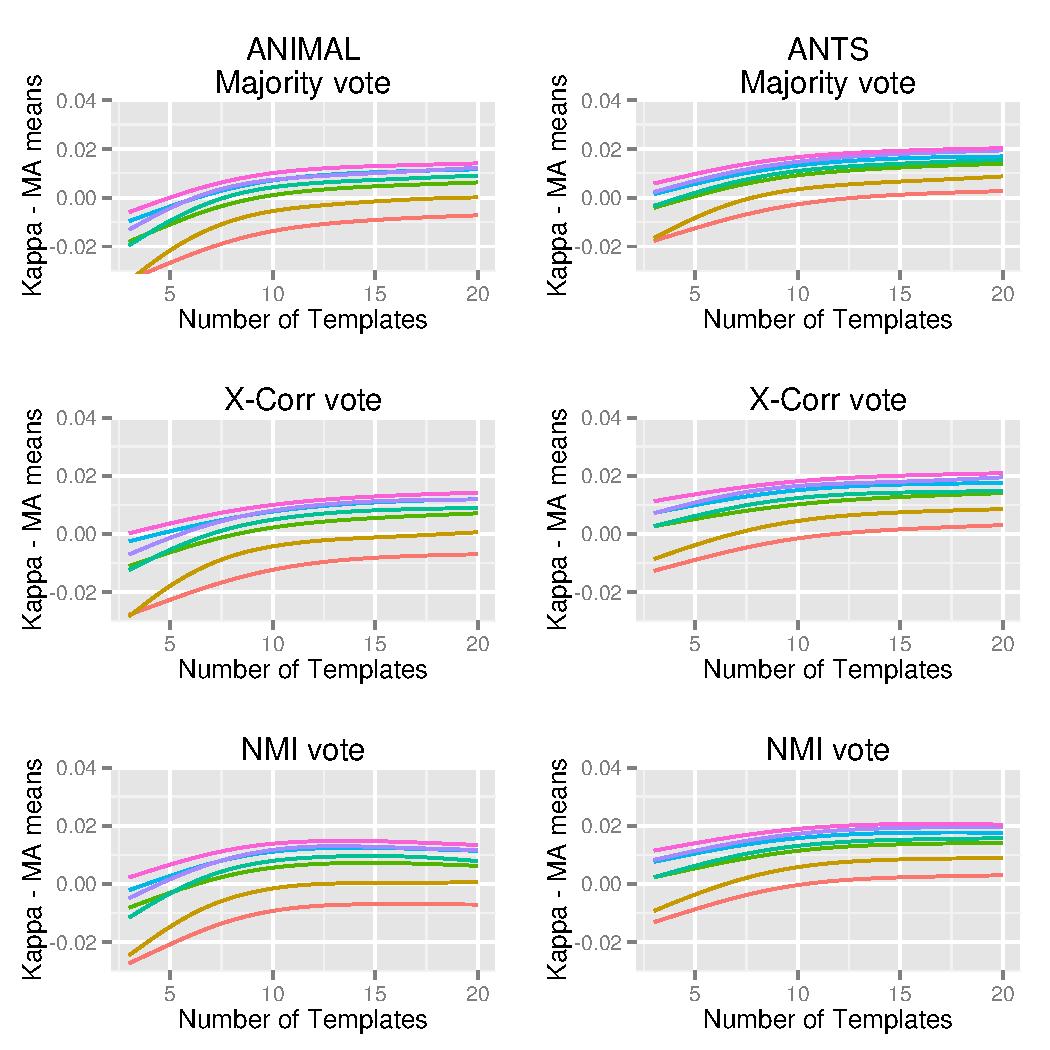
\includegraphics[width=\maxwidth]{figure/a2a} 
\end{knitrout}


Kappa minus multi-atlas mean vs. Number of Templates

Multi-atlas means:

\begin{table}
    \begin{tabular}{c|c|c}
        Number of Atlases & ANIMAL Kappa (Jaccard) & ANTS Kappa (Jaccard) \\ \hline
        3                 & 0.76 (0.63)             & 0.80 (0.69)          \\ 
        4                 & 0.75 (0.62)             & 0.79 (0.67)          \\ 
        5                 & 0.79 (0.66)             & 0.82 (0.71)          \\ 
        6                 & 0.78 (0.65)             & 0.82 (0.70)          \\ 
        7                 & 0.80 (0.67)             & 0.83 (0.72)          \\ 
        8                 & 0.79 (0.67)             & 0.83 (0.72)          \\ 
        9                 & 0.80 (0.68)             & 0.84 (0.73)          \\
    \end{tabular}
\end{table}

- more atlases -> better performance
- larger template library -> better performance, but tails off around 10-15 templates
- no significant difference between majority or weighted vote methods (haven’t tested this statistically though). 
- consistently performs better than average naive performance by XXX
- using ANTS, with a large enough template library (>12) MAGeT brain performs better than the average multi-atlas approach with the same number of atlases.  using ANIMAL, 5 or more atlases needed before boost seen. 
- more atlases -> smaller template library required to improve on average multi-atlas performance
- discuss variance?  best/worst case? --how often do we expect random template library selection to work decently

\todo{cost (in registrations) / benefit trade off graph:  show number of registrations per Kappa?  or hours of manual labour per Kappa?)}

\subsubsection{Winterburn Atlas Segmentation of ADNI Baseline Images}

- A2A shows that if atlas population strongly(?) represents subject set variability, then free choice from atlas population will produce improvements (we know this b/c of extensive validation trials). 
- what about in the case where atlas population doesn’t strongly represent subject set variability (e.g. a priori atlas set)?  then, we can use atlas selection to refine atlas set? 

\todo{Kappa against our manual rater is low}




\begin{figure}[h]
\begin{knitrout}
\definecolor{shadecolor}{rgb}{0.969, 0.969, 0.969}\color{fgcolor}

{\centering 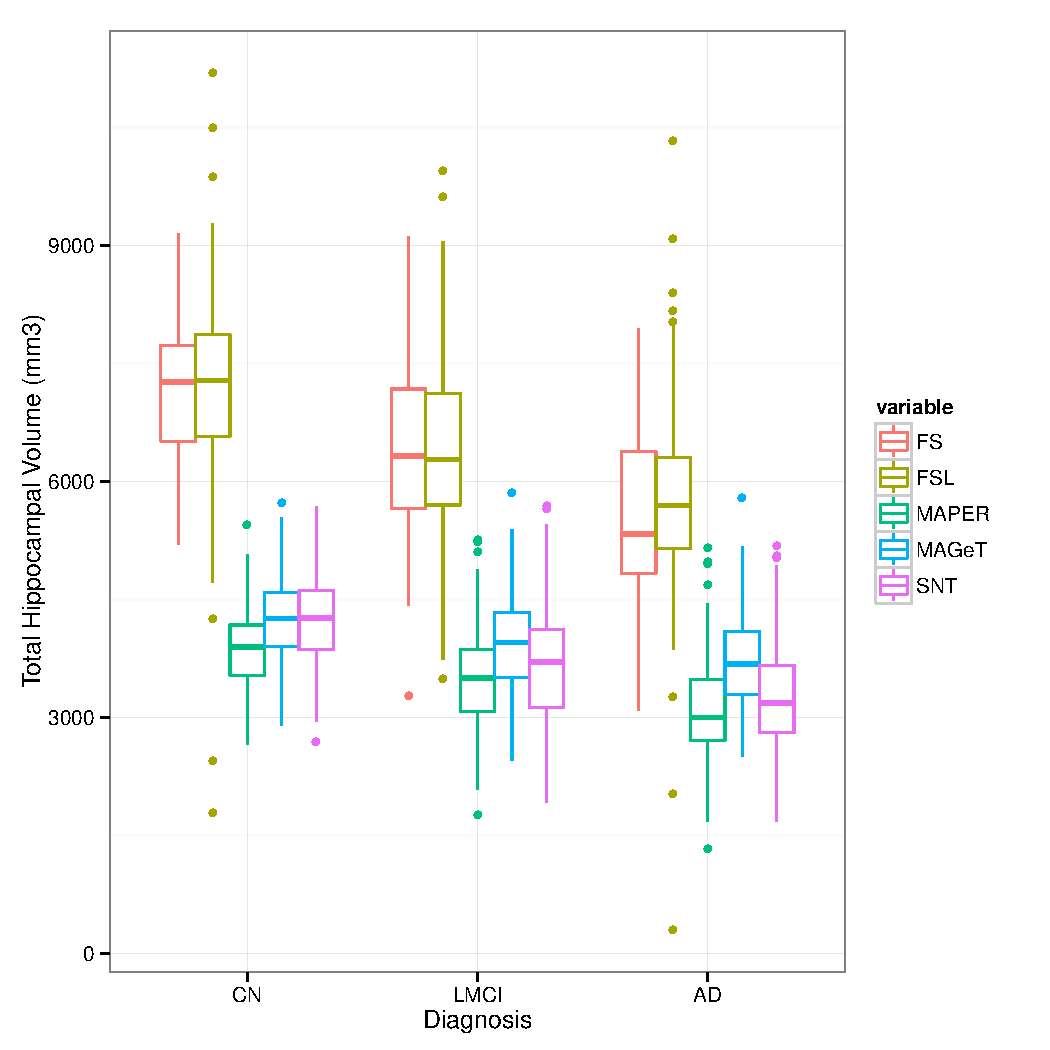
\includegraphics[width=\maxwidth]{figure/ADNI-baseline-volumes-boxplot} 

}


\end{knitrout}

  \caption{Comparison of HC volumes by FreeSurfer (FSF), MAGeT brain (MAGeT), MAPER, and manual (SNT).}
  \label{ADNI-baseline-volumes-boxplot}
\end{figure}

\begin{figure}[h]
\begin{knitrout}
\definecolor{shadecolor}{rgb}{0.969, 0.969, 0.969}\color{fgcolor}\begin{kframe}


{\ttfamily\noindent\textcolor{warningcolor}{\#\# Warning: Removed 359 rows containing missing values (stat\_smooth).}}

{\ttfamily\noindent\textcolor{warningcolor}{\#\# Warning: Removed 355 rows containing missing values (stat\_smooth).}}

{\ttfamily\noindent\textcolor{warningcolor}{\#\# Warning: Removed 355 rows containing missing values (stat\_smooth).}}\end{kframe}

{\centering 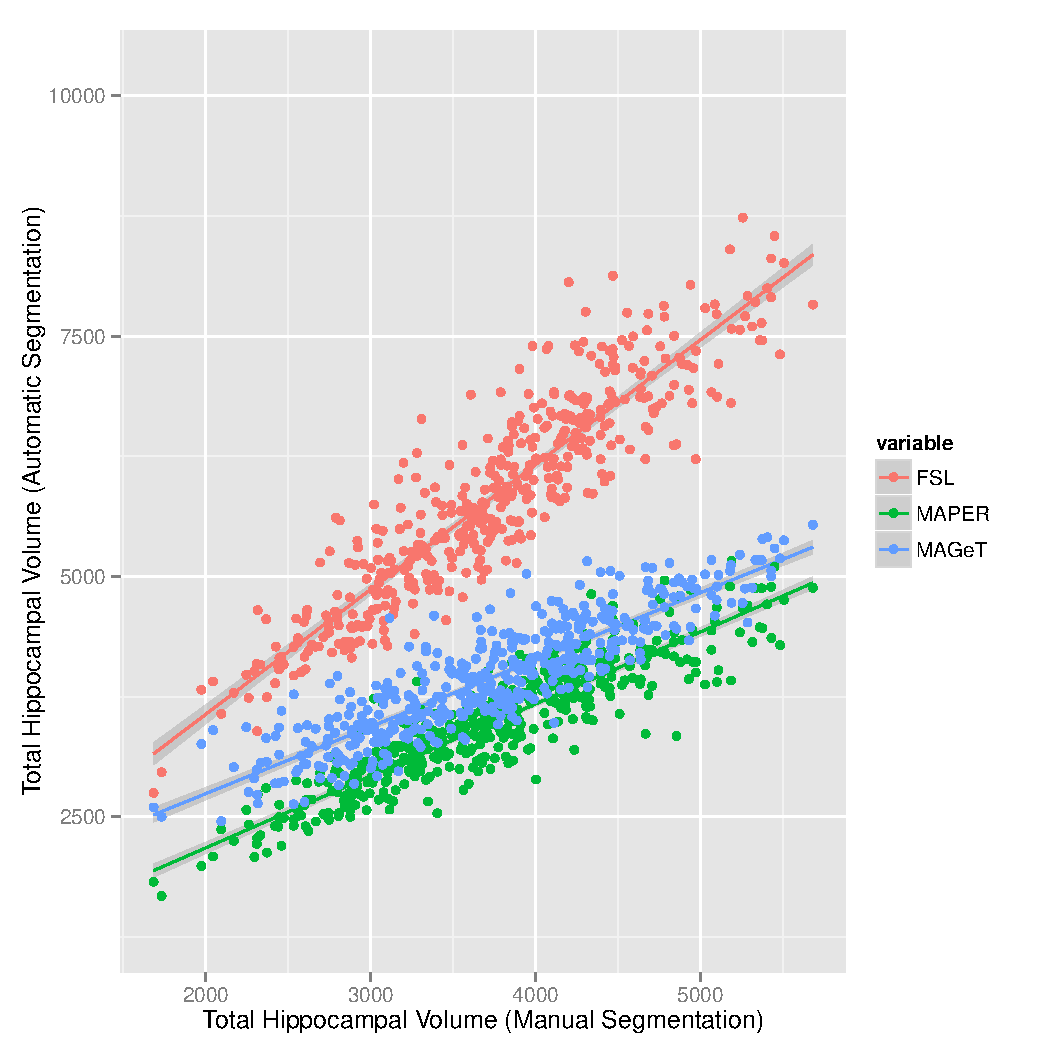
\includegraphics[width=\maxwidth]{figure/ADNI-baseline-volumes-plot} 

}


\end{knitrout}

  \caption{Comparison of HC volumes by FreeSurfer (FSF), MAGeT brain (MAGeT), MAPER, and manual (SNT).}
  \label{ADNI-baseline-volumes-plot}
\end{figure}

\end{document}
